\section*{Morphological Processing}

\textbf{Morphological image processing} (or morphology) describes a
range of image processing techniques that deal with the shape (or
morphology) of features in an image.

Morphological operations are typically applied to remove
imperfections introduced during segmentation, and so typically
operate on bi-level images

\subsection*{Structuring Elements, Hits and Fits}

Small binary image which defines the shape of the operation, similar
to a convolution kernel.

Structuring elements can be of any shape and size, typically we use
rectangular images with origin at the \textbf{middle pixel}.

\begin{figure}[H]
  \centering
  \includegraphics[width=0.5\linewidth]{images/hits_and_fits.png}
  \caption{$A \rightarrow$ fit, $B \rightarrow$ hit, $C \rightarrow$ miss}
\end{figure}

\subsection*{Erosion}

$f \ominus s \rightarrow$ erosion of image $f$ by structuring element $s$.

$s$ is positioned with origin at $(x, y)$ and the new pixel value becomes:

\begin{equation*}
  g(x, y) =
  \begin{cases}
    1 & \text{if } s \text{ fits } f\\
    0 & \text{otherwise}.
  \end{cases}
\end{equation*}

\begin{figure}[H]
  \centering
  \includegraphics[width=\linewidth]{images/erosion.png}
  \includegraphics[width=0.18\linewidth]{images/erosion_structuring_element.png}
  \caption{Erosion of a binary image with a plus shaped structuring element; note: \textbf{the boundary shrinks}!}
\end{figure}

\subsubsection*{Applications}

\begin{itemize}
  \item Erosion separates \textbf{joined objects}.

    \begin{minipage}{\linewidth}
      \begin{figure}[H]
        \centering
        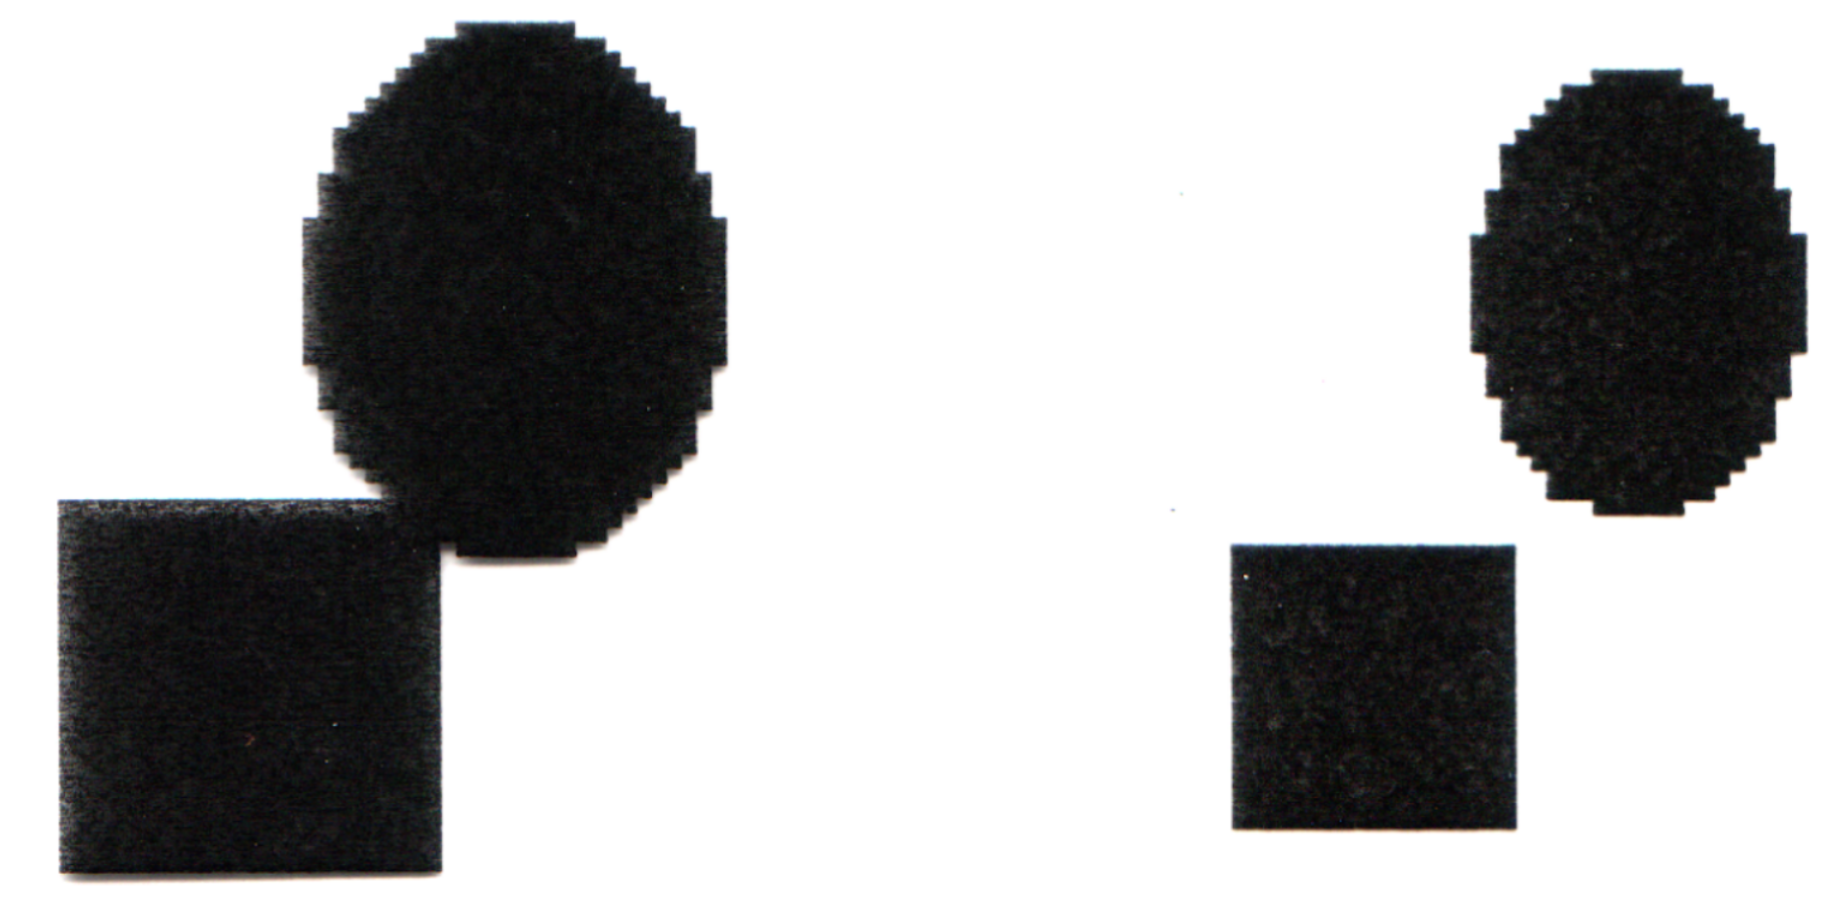
\includegraphics[width=0.7\linewidth]{images/erosion_joined_objects.png}
      \end{figure}
    \end{minipage}

  \item Erosion removes \textbf{extrusions}.

    \begin{minipage}{\linewidth}
      \begin{figure}[H]
        \centering
        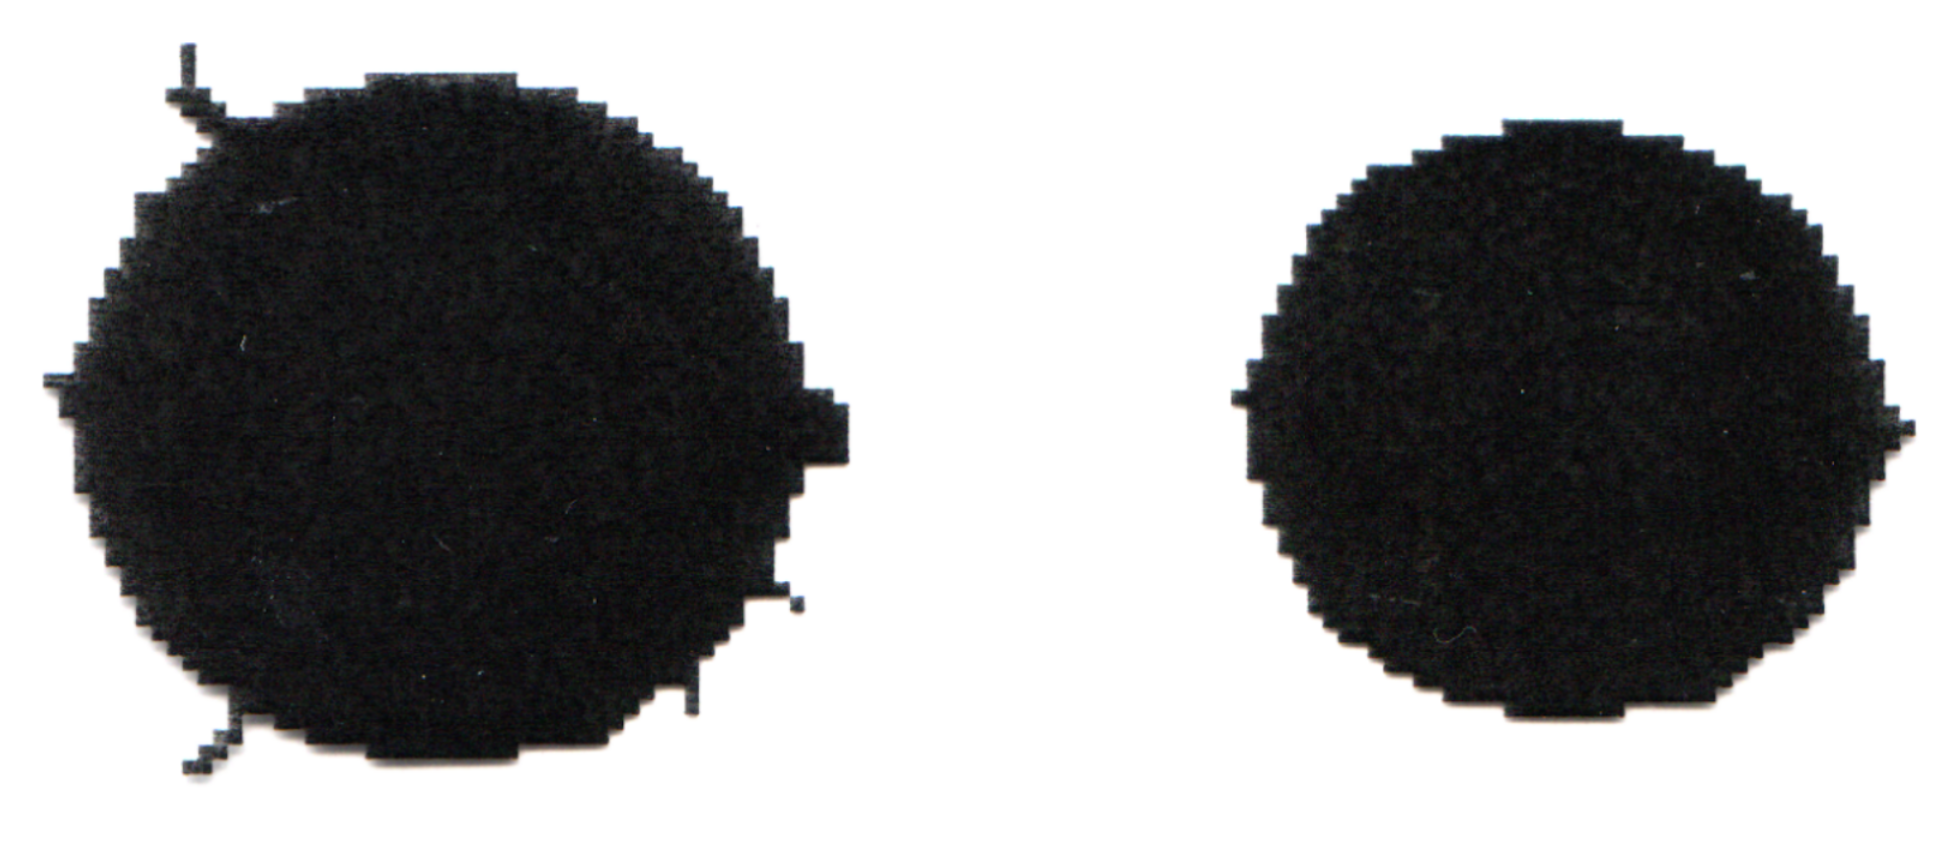
\includegraphics[width=0.7\linewidth]{images/erosion_extrusions.png}
      \end{figure}
    \end{minipage}
\end{itemize}    

\subsection*{Dilation}

$f \oplus s \rightarrow$ dilation of image $f$ by structuring element $s$.

$s$ is positioned with origin at $(x, y)$ and the new pixel value becomes:

\begin{equation*}
  g(x, y) =
  \begin{cases}
    1 & \text{if } s \text{ hits } f\\
    0 & \text{otherwise}.
  \end{cases}
\end{equation*}

\begin{figure}[H]
  \centering
  \includegraphics[width=\linewidth]{images/dilation.png}
  \includegraphics[width=0.18\linewidth]{images/dilation_structuring_element.png}
  \caption{Dilation of a binary image with a plus shaped structuring element; note: \textbf{the boundary expands}!}
\end{figure}

\subsubsection*{Applications}

\begin{itemize}
  \item Dilation can \textbf{repair breaks}

    \begin{minipage}{\linewidth}
      \begin{figure}[H]
        \centering
        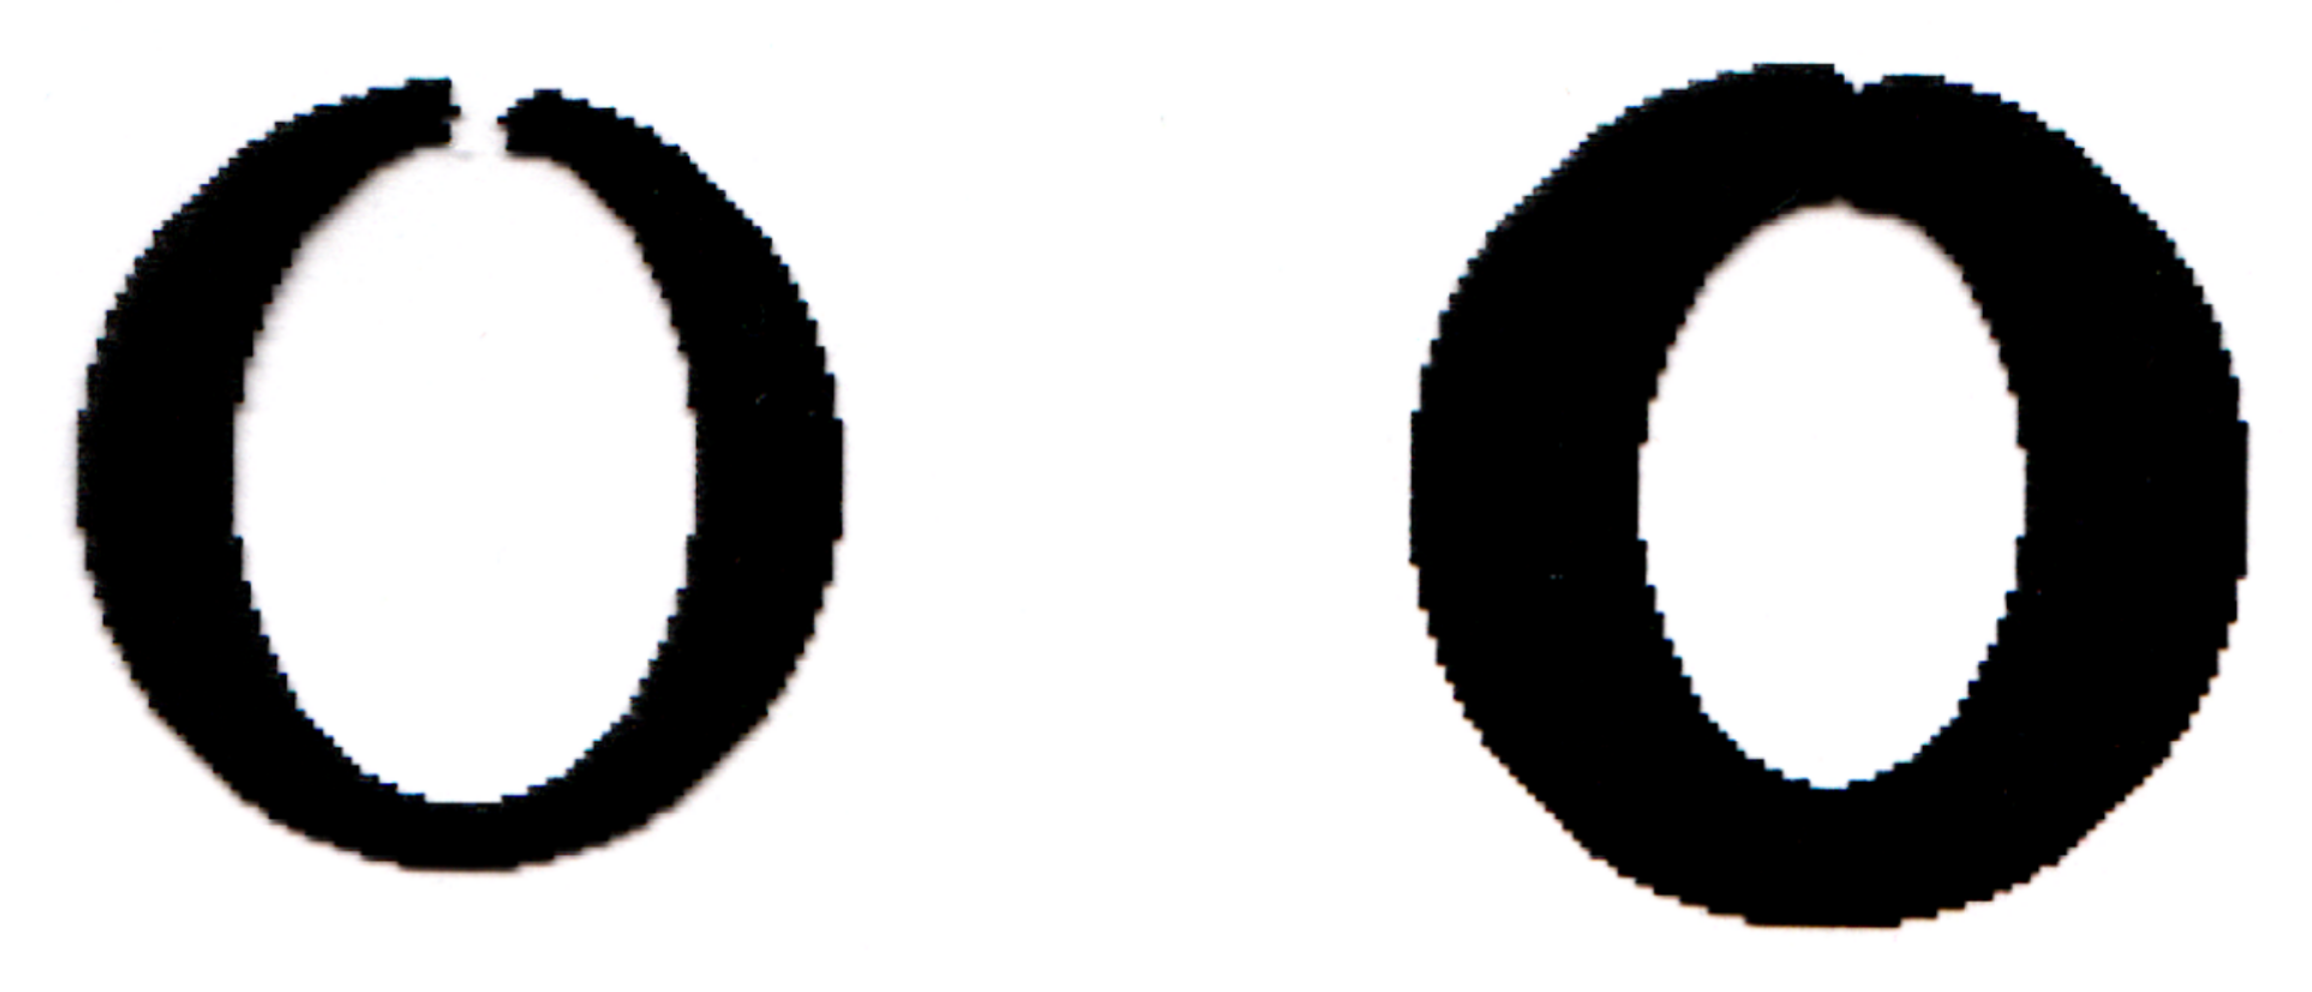
\includegraphics[width=0.7\linewidth]{images/dilation_repair_breaks.png}
      \end{figure}
    \end{minipage}

  \item Dilation can repair \textbf{intrusions}

    \begin{minipage}{\linewidth}
      \begin{figure}[H]
        \centering
        
\includegraphics[width=0.7\linewidth]{images/dilation_repair_intrusions.png}
      \end{figure}
    \end{minipage}
\end{itemize}
  

\subsection*{Opening}

\textbf{Compound operation} of erosion followed by dilation. Separates objects while preserving their size.

\begin{equation*}
  f \circ s = (f \ominus s) \oplus s
\end{equation*}

\begin{figure}[H]
  \centering
  \includegraphics[width=\linewidth]{images/opening.png}
  \includegraphics[width=0.18\linewidth]{images/opening_structuring_element.png}
  \caption{Opening of a binary image with a plus shaped structuring element}
\end{figure}

\subsection*{Closing}

\textbf{Compound operation} of dilation followed by erosion. Fills small holes while preserving the size of objects.

\begin{equation*}
  f \bullet s = (f \oplus s) \ominus s
\end{equation*}

\begin{figure}[H]
  \centering
  \includegraphics[width=\linewidth]{images/closing.png}
  \includegraphics[width=0.18\linewidth]{images/closing_structuring_element.png}
  \caption{Closing of a binary image with a plus shaped structuring element}
\end{figure}

\textbf{Note}: \enquote{Morphological open-close} is a fairly common operation, which is simply \textbf{opening followed by closing}.

\subsection*{Region Filling}

\textbf{Goal:} Given a pixel inside a boundary, attempt to fill the boundary with \textbf{object pixels} (1's).

\begin{equation*}
  X_k = (X_{k-1} \oplus B) \cap A^c
\end{equation*}

$k = 1, 2, \ldots 3$

(i) $X_0 \rightarrow$ simply the starting point inside the boundary, (ii) $B \rightarrow$ simple structuring element and (iii) $A^c \rightarrow$ complement of A

Equation's applied repeatedly until $X_k$ is equal to $X_{k-1}$

\begin{figure}[H]
  \centering
  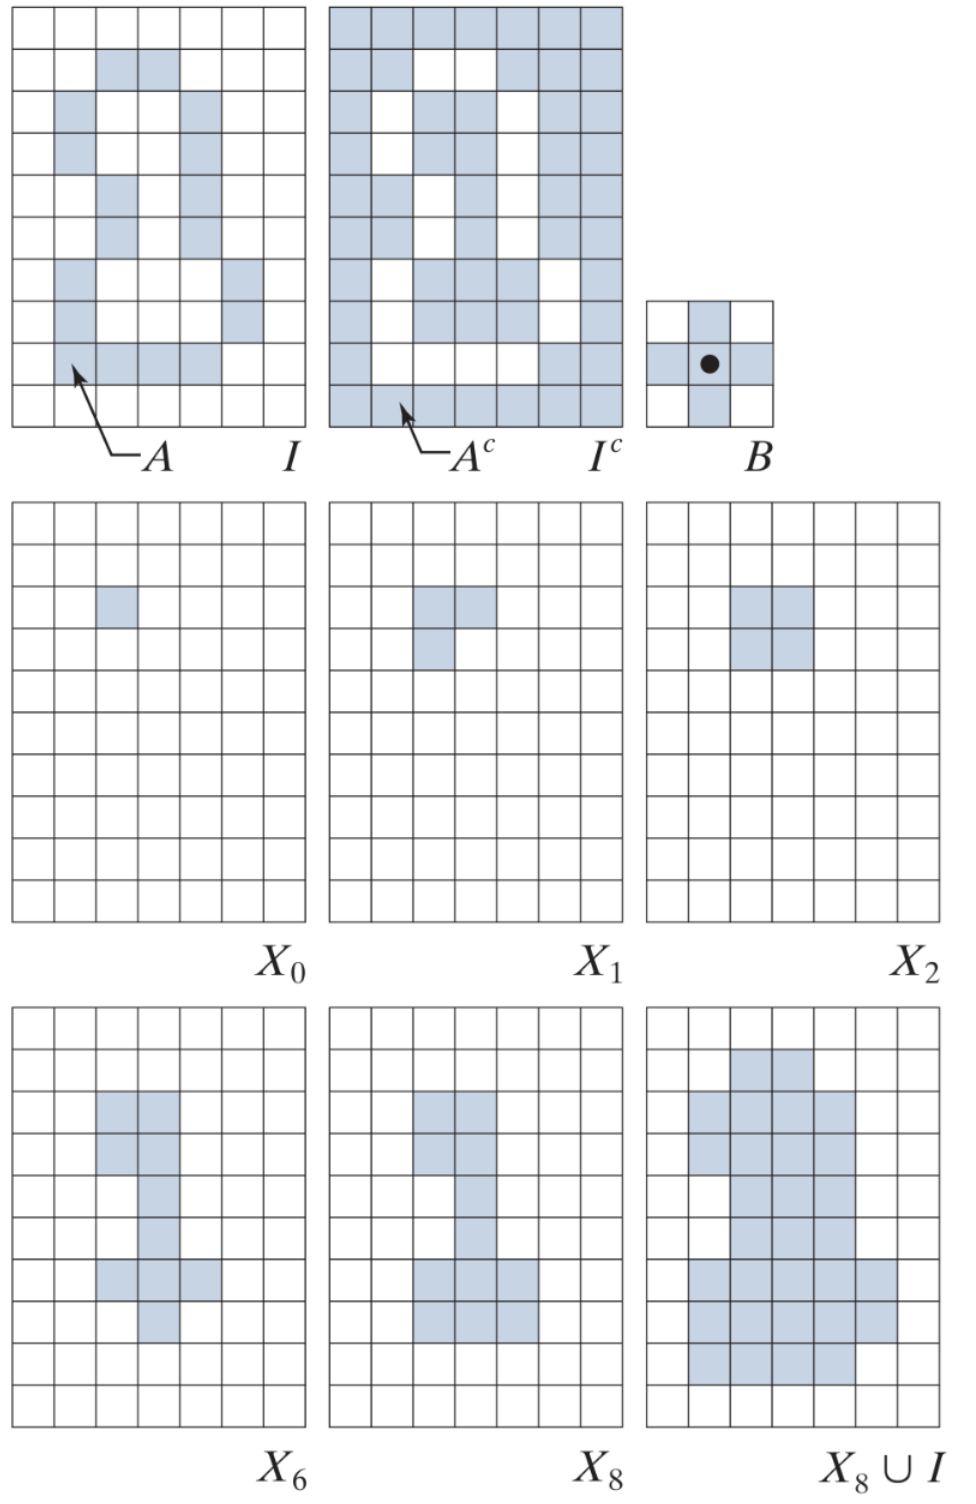
\includegraphics[width=\linewidth]{images/region_filling.png}
  \caption{Region filling example}
\end{figure}

\subsubsection*{Applications}
\begin{itemize}
  \item Forensic and biometric fingerprint enhancement: filling spurious gaps in binarized fingerprint images, ensuring continuous ridge structures
  \item Filling in concavities in CT images (such as pleural lesions and eliminate internal cavities caused by respiratory motion specifically in pulmonary CT images) prior to segmentation
\end{itemize}

\subsection*{Boundary Extraction}

The boundary is simply given by:

\begin{equation*}
  \beta(A) = A - A \ominus B
\end{equation*}

\textbf{Intuition:} $A \ominus B$ removes the boundary of $A$ by eroding it with $B$, and then we subtract the eroded image from the original image to get the boundary.

\begin{figure}[H]
  \centering
  \includegraphics[width=\linewidth]{images/boundary_extraction.png}
  \caption{Boundary extraction example}
\end{figure}

\subsubsection*{Applications}

\begin{itemize}
  \item Optical Character Recognition (OCR) preprocessing: to delineate the contours of text characters, enabling accurate segmentation of connected characters before recognition
  \item Isolating inner and outer boundaries of blood vessel walls in vascular images; useful for measuring arterial lumen and wall thickness
\end{itemize}
